La concentrazione di una soluzione è la grandezza che esprime il rapporto tra la quantità di soluto e la quantità di solvente.
\subsection{Modi di esprimere la concentrazione}
La concentrazione può essere espressa in diversi modi:
\subsubsection{Percentuale in massa}
Con questo metodo si ottiene un numero adimensionale definito come

$$ \frac{\text{grammi di soluto}}{100\text{ grammi di soluzione}} \cdot 100$$

Va da notare che nei 100g di soluzione sono sommati solvente e soluto. Ciò nella pratica corrispondere a prendere un certo numero di grammi di soluto e aggiungere grammi di solvente fino ad arrivare a 100g.
\subsubsection{Percentuale in volume}
\E definita come

$$ \frac{\text{mL di soluto}}{100\text{ mL di soluzione}} \cdot 100$$

\subsubsection{Frazione molare}
\E un rapporto tra le moli di un qualunque componente della soluzione diviso la somma delle moli totali. Nel caso di una soluzione di due sole componenti A e B la frazione molare, indicata con $\rchi$, sarà

$$\rchi_A=\frac{n_A}{n_A + n_B}
\qquad
\rchi_B=\frac{n_B}{n_A + n_B}
\qquad
\rchi_A + \rchi_B = 1$$

\E insito nella definizione che la somma delle frazioni molari sarà sempre uguale a 1.
\subsubsection{Molarità (M)}
Si definisce come le moli di soluto in un litro di soluzione. Va da notare che avremo così moli su volume. Ciò nella pratica corrisponde, ad esempio, ad avere un contenitore di cui conosciamo il volume, mettiamo un certo numero di grammi di NaCl (che è il soluto) che corrisponderanno ad un certo numero di moli e poi aggiungiamo H$_2$O (che è il solvente) fin quando il volume totale (dato sia da solvente che soluto) equivale a 1L (quindi NO certe moli + 1L di acqua).
\subsubsection{Molalità (m)}
Si definisce come le moli di soluto in 1000 grammi di solvente puro (e non di soluzione!). Ciò significa che in questo caso se ad esempio aggiungiamo una certa quantità di grammi di NaCl ne dovremo poi aggiungere 1000 di H$_2$O,per cui il volume finale sarà più di 1L e la massa della soluzione sarà più di 1000 grammi.

Molarità e molalità sono quindi molto diverse.
\subsubsection{Normalità (N)}
Si definisce come gli equivalenti di soluto in 1L di soluzione.

La definizione è identica a quella della molarità tranne per il fatto che al posto delle moli abbiamo gli equivalenti. Cosa sono questi?

Le moli sono definite come grammi su peso molecolare (g/MM), gli equivalenti come grammi su peso equivalente (g/ME). Il peso equivalente è il peso molecolare diviso un numero. Di volta in volta bisogna vedere a quale reazione stia partecipando quel composto e cosa succede. In particolare:
\begin{itemize}
    \item Negli acidi il numero per cui bisogna dividere corrisponde al numero di protoni (cioè ioni H$^+$) che liberano a seguito della dissociazione;
    \item Nelle basi è pari al numero di ioni OH$^-$ che liberano a seguito della dissociazione;
    \item In una reazione redox è il numero di elettroni scambiati da quella specie.
    \item Nel caso di una dissociazione di un sale è il numero delle cariche positive (o negative) prodotte dalla dissociazione.
\end{itemize}

Per capire meglio facciamo degli esempi:

\begin{enumerate}
    \item \textbf{Acido cloridrico HCl}
    
    Esso in acqua si dissocia in H$^+$ e Cl$^-$. Quindi si produce uno ione da una molecola di HCl. In questo caso peso molecolare e equivalente coincidono, per cui molarità e normalità saranno la stessa cosa;
    \item \textbf{Idrossido di sodio NaOH}
    
    Esso in acqua si dissocia in Na$^+$ e OH$^-$. Quindi da una unità formula (per le speci ioniche non esistono le molecole) di NaOH in soluzione si ottiene uno ione, per cui il rapporto è 1:1. Pertanto anche in questo caso peso molecolare e equivalente coincidono, cioè molarità e normalità sono uguali.
    \item \textbf{Acido solforico $\mathbf{H_2SO_4}$}
    
    Esso in acqua si dissocia liberando due ioni H$^+$ ed uno ione SO$_4^{2-}$. Quindi per ogni molecola di H$_2$SO$_4$ in soluzione otterremo due ioni $\rm H^+$. Allora in questo caso il peso equivalente sarà dato dal peso molecolare diviso due, cioè il peso equivalente è la metà. Quindi se il peso molecolare dell'H$_2$SO$_4$ è circa 98, il peso equivalente è circa 49, per cui se avessimo 98 grammi di acido solforico diremmo di averne una mole (98/98=1), mentre per ottenere gli equivalenti dovremmo dividere per 49 e quindi avremmo 2 equivalenti. Si può anche dire che una mole di H$_2$SO$_4$ messa in un litro d'acqua dà una soluzione 1-molare o 2-normale.

    Quindi, siccome l'acido solforico dà due protoni in soluzione, la normalità è il doppio della molarità
    \item \textbf{Idrossido di calcio $\mathbf{Ca(OH)_2}$}
    
    Esso in acqua si dissocia in Ca$^{2+}$ più due ioni OH$^-$. Ne segue che in questo caso il peso equivalente è la metà del peso molecolare, quindi la normalità del Ca(OH)$_2$ è il doppio della sua molarità (in un caso dividiamo per 74, nell'altro per 37).
    \item \textbf{Permanganato di potassio KMnO$_{\boldsymbol{4}}$}
    
    Esso può nascere da diverse ossidoriduzioni. Se si trova in ambiente fortemente acido il manganese del permanganato si comporterà da ossidante e passerà da stato di ossidazione +7 a stato di ossidazione +2 con l'acquisto di 5 elettroni ($\ce{Mn^{7+} + 5e -> Mn^{2+}}$). Il peso equivalente sarà uguale al peso molecolare diviso 5, cioè avremo M.M.=158 e M.E.=31.6.

    Quindi una soluzione 1-molare di KMnO$_4$ sarà 5-normale, nel caso in cui stiamo operando una redox ed il manganese va da +7 a +2. 
    
    \vspace{0.2cm}Se invece ci troviamo in ambiente poco acido, si otterrà l'MnO$_2$ e quindi il manganese passa da stato di ossidazione +7 a stato di ossidazione +4 con l'acquisto di 3 elettroni ($\ce{Mn^{7+} + 3e -> Mn^{4+}}$), per cui il peso equivalente sarà pari al peso molecolare diviso 3.

    \E dunque fondamentale capire in quale reazione si trova il composto e cosa sta dando luogo.

    \item \textbf{Solfato ferrico $\mathbf{Fe_2(SO_4)_3}$}

    Esso si dissocia in due ioni $\rm Fe^{3+}$ e tre ioni $\rm SO_4^{2-}$. Complessivamente vengono liberate 6 cariche positive (o 6 cariche negative), per cui il peso equivalente sarà pari al peso molecolare diviso 6, cioè avremo M.M.=399.88 e M.E.=66.647.
\end{enumerate}

Da questi esempi deduciamo che tutti gli acidi monoprotici e tutte le basi monoprotiche (cioè che cedono un solo ione) hanno peso molecolare e peso equivalente identici, mentre in generale acidi n-protici e basi n-protiche hanno peso equivalente pari al peso molecolare diviso n.

\E chiaro che il peso equivalente è sempre minore o uguale al peso molecolare e quindi a parità di grammi il numero di equivalenti è maggiore o uguale al numero di moli perché dividiamo i grammi per un numero minore o uguale.

\hspace{1cm}\begin{minipage}{0.42\textwidth}
    \begin{figure}[H]
        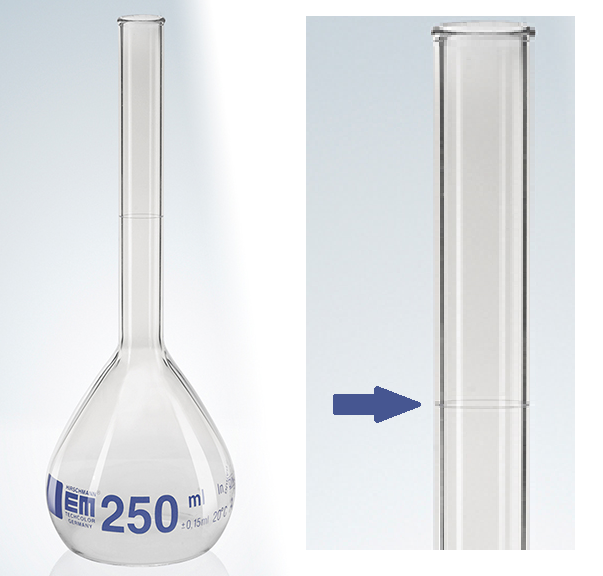
\includegraphics[width=6cm]{immagini/matraccio.png}
    \end{figure}
\end{minipage}
\begin{minipage}{0.5\textwidth}
    Ci sono vari modi per essere precisi nella misura di un volume. Uno di questi consiste nell'adoperare un matraccio, che è un contenitore come in figura che se riempito fino ad una certa tacca mostra un "menisco", ossia la superficie del liquido avrà una forma concava che ci permette di essere variare il volume a passi di una goccia, che equivale a 0.005 mL.
\end{minipage}

\vspace{0.4cm}L'operazione che si fa in laboratorio quando si prepara una soluzione è prendere il contenitore, mettere un po' di solvente, poi aggiungere il soluto e infine si riaggiunge il solvente fino al volume desiderato. Conviene fare così anziché mettere prima il soluto e poi tutto il solvente perché le reazioni di solvatazione sono esotermiche. Se quindi abbiamo già del solvente e poi aggiungiamo del soluto, quando questo passa in soluzione e sviluppa calore quest'ultimo verrà assorbito dal solvente già presente; se invece non mettessimo preliminarmente del solvente, non appena lo aggiungiamo partirà il processo di solvatazione sviluppando calore, ma non avendo abbastanza solvente che lo assorba il calore verrà dissipato attraverso il vetro causando la rottura del contenitore.

\vspace{0.2cm}Vediamo ora un esempio pratico.

Immaginiamo di avere 2mL di acido solforico H$_2$SO$_4$, la cui densità è pari a 1.9 g/mL. Supponiamo di voler aggiungere ad essi acqua fino ad arrivare a 100 mL.

Vogliamo calcolare:

\vspace{0.2cm}a) La percentuale in massa;

\vspace{0.2cm}b) La percentuale in volume;

\vspace{0.2cm}c) Le frazioni molari;

\vspace{0.2cm}d) La molalità $m$;

\vspace{0.2cm}e) La molarità $M$;

\vspace{0.2cm}f) La normalità $N$.

\vspace{0.2cm}Innanzitutto calcoliamo le varie quantità che ci serviranno.

Per arrivare a 100 mL di soluzione, dato che abbiamo già 2 mL di H$_2$SO$_4$ dovremo aggiungere 98 mL di acqua.

I grammi contenuti in 2 mL di H$_2$SO$_4$ sono
$$g_{\text{H}_2\text{SO}_4}=V\cdot d_{\text{H}_2\text{SO}_4}= 2 \cdot 1.9=3.8$$
Nota: come unità di misura della densità useremo g/mL per i liquidi e g/L per i gas.

I grammi necessari saranno
$$g_{\text{H}_2\text{O}}= V \cdot d_{\text{H}_2\text{O}}= 98 \cdot 1 = 98$$
Calcoliamo le moli
$$n_{\text{H}_2\text{SO}_4}=\frac{g}{M.M.}=\frac{3.8}{98.074}=0.038746=3.8746 \cdot 10^{-2}$$
$$n_{\text{H}_2\text{O}}=\frac{g}{M.M.}=\frac{98}{18.0528}=5.4398$$
In questo modo potremo avere le moli totali.

\vspace{0.2cm}a) Per calcolare la percentuale in massa troviamo la massa totale:
$$m_{tot}=3.8 + 98=101.8 \; \text{grammi}
\implies \frac{3.8}{101.8} \cdot 100 = 3.73 \%$$
b) La percentuale in volume sarà
$$\frac{V_{\text{H}_2\text{SO}_4}}{V_{tot}} \cdot 100= \frac{2}{100} \cdot 100 = 2 \%$$
c) Per le frazioni molari calcoliamo prima le moli totali
$$n_{tot}=n_{\text{H}_2\text{SO}_4} + n_{\text{H}_2\text{O}}=0.038746 + 5.4398= 5.4785$$
$$\implies \rchi_{\text{H}_2\text{SO}_4}=\frac{0.038746}{5.4785}=0.00707237
\qquad
\rchi_{\text{H}_2\text{O}}=\frac{5.4398}{5.4785}=0.992936$$

\vspace{0.2cm}A conferma della correttezza dei calcoli si ha che $\rchi_{\text{H}_2\text{SO}_4} + \rchi_{\text{H}_2\text{O}} \approx 1$.

\vspace{0.2cm}d) Per la molalità dobbiamo fare una proporzione perché abbiamo le moli di H$_2$SO$_4$ in 98 grammi di solvente puro, mentre a noi serve il numero di moli in 1000 grammi:
$$n_{\text{H}_2\text{SO}_4}:98 \; g = m :1000 \; g
\implies m = \frac{0.038746}{98} \cdot 1000
\approx 0.39537= 3.9537 \cdot 10^{-1}$$
Il valore trovato per $m$ dovrà essere leggermente diverso rispetto a quello che troveremo per $M$.

\vspace{0.2cm}e) Anche per la molarità bisogna fare una proporzione, che stavolta sarà del tipo
$$n_{\text{H}_2\text{SO}_4}: 100 \; mL = M :1000 \; mL
\implies 
M=\frac{0.038746}{100} \cdot 1000 = 0.38746$$
Tale valore differisce leggermente da quello della molalità perché quella era il numero di moli in 98 grammi di solvente puro, mentre questa è il numero di moli in 100 mL di soluzione.

\vspace{0.2cm}N.B.: $M$ ci dà il numero corrispondente di moli se il volume finale della soluzione è 1000 mL. Ciò significa che la molarità è subito calcolabile come il rapporto tra il numero di moli ed il volume espresso in litri, ossia
$$M=\frac{n}{V(L)}=\frac{0.038746}{0.1}$$
f) Per la normalità dobbiamo innanzitutto osservare che l'acido solforico ha due protoni, per cui quando si dissocia dà luogo a due ioni H$^+$ e uno ione SO$_4^{2-}$. Immaginando che ogni molecola di H$_2$SO$_4$ liberi entrambi i protoni in soluzione, il peso equivalente sarà uguale al peso molecolare diviso due, cioè sarà 49 anziché 98. Ne segue che il numero di equivalenti sarà il doppio del numero di moli:
$$M.E.=\frac{M.M.}{2} \implies n_E=n \cdot 2 = 0.038746 \cdot 2 = 0.077492$$
La normalità allora sarà pari alla molarità per due:
$$N=\frac{0.077492}{0.100}=0.77492 \implies N=M \cdot 2$$
\newpage